\section{Introduction}

For the Real-time Operating Systems course (ROS01) taught at Rotterdam University of Applied Science,
the authors had to implement a scheduler for a Real-time Operating System developed by one lecturers.
Because these types of programming issues like implementing a scheduler require the programmer to be able to program at a low level and it cannot be assumed that every student following this course is familiar with low level progamming (both in the C programming language and assembler), this course contains multiple assingments to bridge this gap.
The code has been flashed and tested on the CC3220s development board (Figure \ref{fig:cc3220s}). The compiler used is TI v18.12.2.LTS.

What's worth mentioning is that some code snippets in this document make a function call to \texttt{delay\_1sec()}.
Because this is used quite a few times and redundant to have multiple definitions in this document its implementation can be seen in Appendix \ref{subsec:appendix_delay}.


\begin{figure}[H]
    \centering

    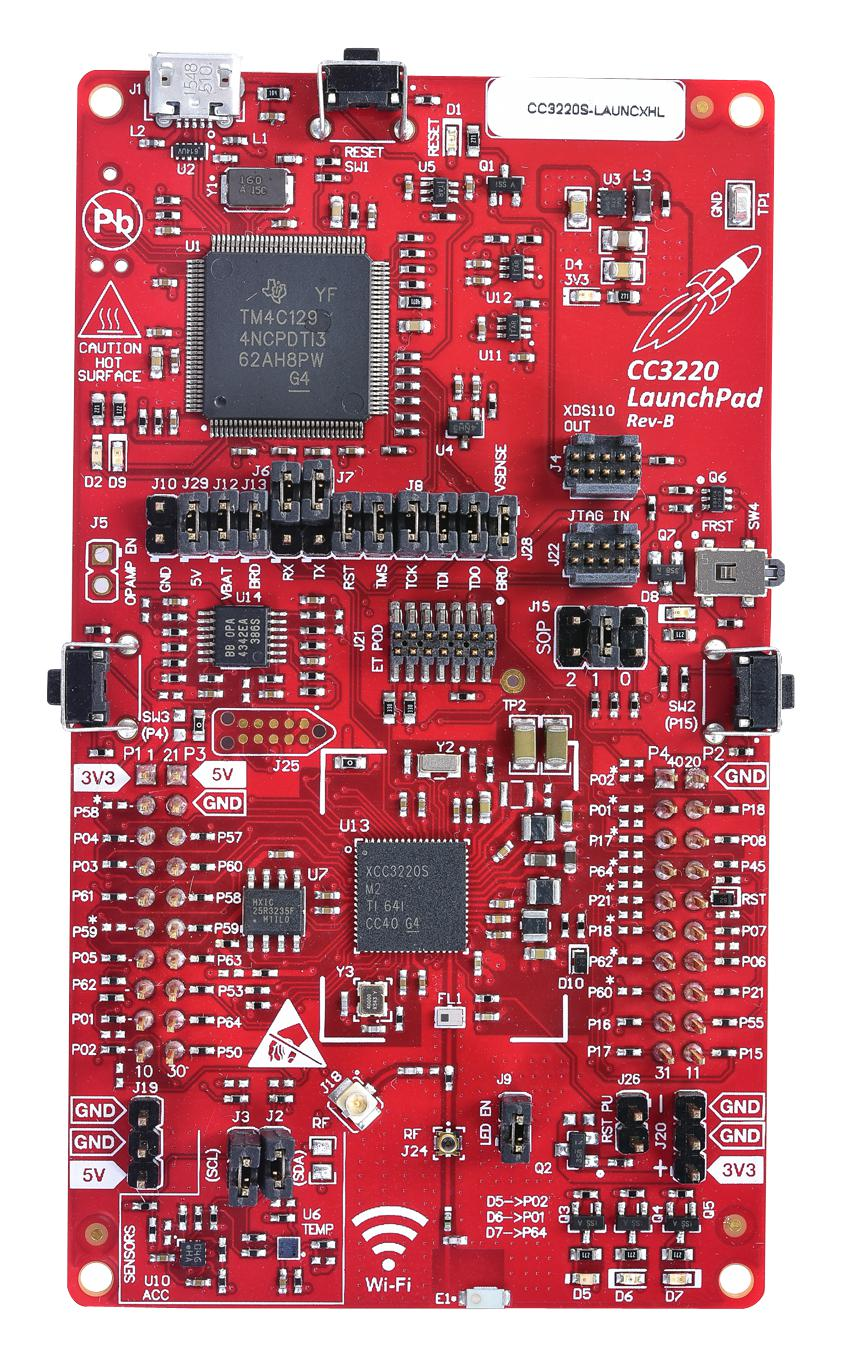
\includegraphics[angle=90,scale=0.2]{img/cc3220s.jpg}

    \caption{Foo}
    \label{fig:cc3220s}

\end{figure}
